\documentclass[]{article}
\usepackage{lmodern}
\usepackage{amssymb,amsmath}
\usepackage{ifxetex,ifluatex}
\usepackage{fixltx2e} % provides \textsubscript
\ifnum 0\ifxetex 1\fi\ifluatex 1\fi=0 % if pdftex
  \usepackage[T1]{fontenc}
  \usepackage[utf8]{inputenc}
\else % if luatex or xelatex
  \ifxetex
    \usepackage{mathspec}
  \else
    \usepackage{fontspec}
  \fi
  \defaultfontfeatures{Ligatures=TeX,Scale=MatchLowercase}
\fi
% use upquote if available, for straight quotes in verbatim environments
\IfFileExists{upquote.sty}{\usepackage{upquote}}{}
% use microtype if available
\IfFileExists{microtype.sty}{%
\usepackage{microtype}
\UseMicrotypeSet[protrusion]{basicmath} % disable protrusion for tt fonts
}{}
\usepackage[margin=1in]{geometry}
\usepackage{hyperref}
\hypersetup{unicode=true,
            pdftitle={Lab Assignment 4: Pokemon Challenge},
            pdfborder={0 0 0},
            breaklinks=true}
\urlstyle{same}  % don't use monospace font for urls
\usepackage{color}
\usepackage{fancyvrb}
\newcommand{\VerbBar}{|}
\newcommand{\VERB}{\Verb[commandchars=\\\{\}]}
\DefineVerbatimEnvironment{Highlighting}{Verbatim}{commandchars=\\\{\}}
% Add ',fontsize=\small' for more characters per line
\usepackage{framed}
\definecolor{shadecolor}{RGB}{248,248,248}
\newenvironment{Shaded}{\begin{snugshade}}{\end{snugshade}}
\newcommand{\KeywordTok}[1]{\textcolor[rgb]{0.13,0.29,0.53}{\textbf{#1}}}
\newcommand{\DataTypeTok}[1]{\textcolor[rgb]{0.13,0.29,0.53}{#1}}
\newcommand{\DecValTok}[1]{\textcolor[rgb]{0.00,0.00,0.81}{#1}}
\newcommand{\BaseNTok}[1]{\textcolor[rgb]{0.00,0.00,0.81}{#1}}
\newcommand{\FloatTok}[1]{\textcolor[rgb]{0.00,0.00,0.81}{#1}}
\newcommand{\ConstantTok}[1]{\textcolor[rgb]{0.00,0.00,0.00}{#1}}
\newcommand{\CharTok}[1]{\textcolor[rgb]{0.31,0.60,0.02}{#1}}
\newcommand{\SpecialCharTok}[1]{\textcolor[rgb]{0.00,0.00,0.00}{#1}}
\newcommand{\StringTok}[1]{\textcolor[rgb]{0.31,0.60,0.02}{#1}}
\newcommand{\VerbatimStringTok}[1]{\textcolor[rgb]{0.31,0.60,0.02}{#1}}
\newcommand{\SpecialStringTok}[1]{\textcolor[rgb]{0.31,0.60,0.02}{#1}}
\newcommand{\ImportTok}[1]{#1}
\newcommand{\CommentTok}[1]{\textcolor[rgb]{0.56,0.35,0.01}{\textit{#1}}}
\newcommand{\DocumentationTok}[1]{\textcolor[rgb]{0.56,0.35,0.01}{\textbf{\textit{#1}}}}
\newcommand{\AnnotationTok}[1]{\textcolor[rgb]{0.56,0.35,0.01}{\textbf{\textit{#1}}}}
\newcommand{\CommentVarTok}[1]{\textcolor[rgb]{0.56,0.35,0.01}{\textbf{\textit{#1}}}}
\newcommand{\OtherTok}[1]{\textcolor[rgb]{0.56,0.35,0.01}{#1}}
\newcommand{\FunctionTok}[1]{\textcolor[rgb]{0.00,0.00,0.00}{#1}}
\newcommand{\VariableTok}[1]{\textcolor[rgb]{0.00,0.00,0.00}{#1}}
\newcommand{\ControlFlowTok}[1]{\textcolor[rgb]{0.13,0.29,0.53}{\textbf{#1}}}
\newcommand{\OperatorTok}[1]{\textcolor[rgb]{0.81,0.36,0.00}{\textbf{#1}}}
\newcommand{\BuiltInTok}[1]{#1}
\newcommand{\ExtensionTok}[1]{#1}
\newcommand{\PreprocessorTok}[1]{\textcolor[rgb]{0.56,0.35,0.01}{\textit{#1}}}
\newcommand{\AttributeTok}[1]{\textcolor[rgb]{0.77,0.63,0.00}{#1}}
\newcommand{\RegionMarkerTok}[1]{#1}
\newcommand{\InformationTok}[1]{\textcolor[rgb]{0.56,0.35,0.01}{\textbf{\textit{#1}}}}
\newcommand{\WarningTok}[1]{\textcolor[rgb]{0.56,0.35,0.01}{\textbf{\textit{#1}}}}
\newcommand{\AlertTok}[1]{\textcolor[rgb]{0.94,0.16,0.16}{#1}}
\newcommand{\ErrorTok}[1]{\textcolor[rgb]{0.64,0.00,0.00}{\textbf{#1}}}
\newcommand{\NormalTok}[1]{#1}
\usepackage{graphicx,grffile}
\makeatletter
\def\maxwidth{\ifdim\Gin@nat@width>\linewidth\linewidth\else\Gin@nat@width\fi}
\def\maxheight{\ifdim\Gin@nat@height>\textheight\textheight\else\Gin@nat@height\fi}
\makeatother
% Scale images if necessary, so that they will not overflow the page
% margins by default, and it is still possible to overwrite the defaults
% using explicit options in \includegraphics[width, height, ...]{}
\setkeys{Gin}{width=\maxwidth,height=\maxheight,keepaspectratio}
\IfFileExists{parskip.sty}{%
\usepackage{parskip}
}{% else
\setlength{\parindent}{0pt}
\setlength{\parskip}{6pt plus 2pt minus 1pt}
}
\setlength{\emergencystretch}{3em}  % prevent overfull lines
\providecommand{\tightlist}{%
  \setlength{\itemsep}{0pt}\setlength{\parskip}{0pt}}
\setcounter{secnumdepth}{0}
% Redefines (sub)paragraphs to behave more like sections
\ifx\paragraph\undefined\else
\let\oldparagraph\paragraph
\renewcommand{\paragraph}[1]{\oldparagraph{#1}\mbox{}}
\fi
\ifx\subparagraph\undefined\else
\let\oldsubparagraph\subparagraph
\renewcommand{\subparagraph}[1]{\oldsubparagraph{#1}\mbox{}}
\fi

%%% Use protect on footnotes to avoid problems with footnotes in titles
\let\rmarkdownfootnote\footnote%
\def\footnote{\protect\rmarkdownfootnote}

%%% Change title format to be more compact
\usepackage{titling}

% Create subtitle command for use in maketitle
\newcommand{\subtitle}[1]{
  \posttitle{
    \begin{center}\large#1\end{center}
    }
}

\setlength{\droptitle}{-2em}

  \title{Lab Assignment 4: Pokemon Challenge}
    \pretitle{\vspace{\droptitle}\centering\huge}
  \posttitle{\par}
    \author{}
    \preauthor{}\postauthor{}
    \date{}
    \predate{}\postdate{}
  

\begin{document}
\maketitle

\section{Load data set}\label{load-data-set}

\begin{Shaded}
\begin{Highlighting}[]
\KeywordTok{library}\NormalTok{(tidyverse)}
\KeywordTok{library}\NormalTok{(dplyr)}

\NormalTok{pokes <-}\StringTok{ }\KeywordTok{read.csv}\NormalTok{(}\StringTok{"https://www.dropbox.com/s/i0lwxgv86eaoq4o/pokemon.csv?dl=1"}\NormalTok{)}
\end{Highlighting}
\end{Shaded}

\section{1. At least one plot, with proper
labels.}\label{at-least-one-plot-with-proper-labels.}

\begin{Shaded}
\begin{Highlighting}[]
\CommentTok{# get to know data}
\KeywordTok{summary}\NormalTok{(pokes)}
\end{Highlighting}
\end{Shaded}

\begin{verbatim}
##      Number            Name         Type_1         Type_2   
##  Min.   :  1   Abomasnow :  1   Water  :105           :371  
##  1st Qu.:181   Abra      :  1   Normal : 93   Flying  : 87  
##  Median :361   Absol     :  1   Grass  : 66   Poison  : 31  
##  Mean   :361   Accelgor  :  1   Bug    : 63   Ground  : 30  
##  3rd Qu.:541   Aegislash :  1   Fire   : 47   Psychic : 27  
##  Max.   :721   Aerodactyl:  1   Psychic: 47   Fighting: 19  
##                (Other)   :715   (Other):300   (Other) :156  
##      Total             HP             Attack          Defense      
##  Min.   :180.0   Min.   :  1.00   Min.   :  5.00   Min.   :  5.00  
##  1st Qu.:320.0   1st Qu.: 50.00   1st Qu.: 53.00   1st Qu.: 50.00  
##  Median :424.0   Median : 65.00   Median : 74.00   Median : 65.00  
##  Mean   :417.9   Mean   : 68.38   Mean   : 75.01   Mean   : 70.81  
##  3rd Qu.:499.0   3rd Qu.: 80.00   3rd Qu.: 95.00   3rd Qu.: 85.00  
##  Max.   :720.0   Max.   :255.00   Max.   :165.00   Max.   :230.00  
##                                                                    
##      Sp_Atk           Sp_Def           Speed          Generation   
##  Min.   : 10.00   Min.   : 20.00   Min.   :  5.00   Min.   :1.000  
##  1st Qu.: 45.00   1st Qu.: 50.00   1st Qu.: 45.00   1st Qu.:2.000  
##  Median : 65.00   Median : 65.00   Median : 65.00   Median :3.000  
##  Mean   : 68.74   Mean   : 69.29   Mean   : 65.71   Mean   :3.323  
##  3rd Qu.: 90.00   3rd Qu.: 85.00   3rd Qu.: 85.00   3rd Qu.:5.000  
##  Max.   :154.00   Max.   :230.00   Max.   :160.00   Max.   :6.000  
##                                                                    
##     Height_m        Weight_kg        Catch_Rate   
##  Min.   : 0.100   Min.   :  0.10   Min.   :  3.0  
##  1st Qu.: 0.610   1st Qu.:  9.40   1st Qu.: 45.0  
##  Median : 0.990   Median : 28.00   Median : 65.0  
##  Mean   : 1.145   Mean   : 56.77   Mean   :100.2  
##  3rd Qu.: 1.400   3rd Qu.: 61.00   3rd Qu.:180.0  
##  Max.   :14.500   Max.   :950.00   Max.   :255.0  
## 
\end{verbatim}

\begin{Shaded}
\begin{Highlighting}[]
\CommentTok{# analysis starts here}
\NormalTok{pokes <-}\StringTok{ }\NormalTok{pokes }\OperatorTok\StringTok{ }
\StringTok{  }\KeywordTok{mutate}\NormalTok{(}
    \DataTypeTok{Catch_Difficulty =} \KeywordTok{case_when}\NormalTok{(}
\NormalTok{      Catch_Rate }\OperatorTok{>}\StringTok{ }\DecValTok{170} \OperatorTok{~}\StringTok{ "Easy"}\NormalTok{,}
      \KeywordTok{between}\NormalTok{(Catch_Rate, }\DecValTok{85}\NormalTok{, }\DecValTok{170}\NormalTok{) }\OperatorTok{~}\StringTok{ "Medium"}\NormalTok{, }
\NormalTok{      Catch_Rate }\OperatorTok{<}\StringTok{ }\DecValTok{85} \OperatorTok{~}\StringTok{ "Hard"}
\NormalTok{    ),}
    \DataTypeTok{Catch_Difficulty =} \KeywordTok{factor}\NormalTok{(Catch_Difficulty, }\DataTypeTok{levels =} \KeywordTok{c}\NormalTok{(}\StringTok{"Easy"}\NormalTok{, }\StringTok{"Medium"}\NormalTok{, }\StringTok{"Hard"}\NormalTok{))}
\NormalTok{  ) }

\NormalTok{pokes }\OperatorTok\StringTok{ }\KeywordTok{count}\NormalTok{(Catch_Difficulty)}
\end{Highlighting}
\end{Shaded}

\begin{verbatim}
## # A tibble: 3 x 2
##   Catch_Difficulty     n
##   <fct>            <int>
## 1 Easy               184
## 2 Medium             117
## 3 Hard               420
\end{verbatim}

\begin{Shaded}
\begin{Highlighting}[]
\NormalTok{pokes }\OperatorTok\StringTok{ }
\StringTok{  }\KeywordTok{group_by}\NormalTok{(Type_}\DecValTok{1}\NormalTok{) }\OperatorTok\StringTok{ }
\StringTok{  }\KeywordTok{summarize}\NormalTok{(}\DataTypeTok{avg_Total =} \KeywordTok{mean}\NormalTok{(Total)) }\OperatorTok\StringTok{ }
\StringTok{  }\KeywordTok{mutate}\NormalTok{(}
    \DataTypeTok{Type_1 =} \KeywordTok{fct_reorder}\NormalTok{(Type_}\DecValTok{1}\NormalTok{, avg_Total)}
\NormalTok{  ) }\OperatorTok
\StringTok{  }\KeywordTok{ggplot}\NormalTok{(}\KeywordTok{aes}\NormalTok{(}\DataTypeTok{x =}\NormalTok{ Type_}\DecValTok{1}\NormalTok{, }\DataTypeTok{y =}\NormalTok{ avg_Total, }\DataTypeTok{fill =}\NormalTok{ Type_}\DecValTok{1}\NormalTok{)) }\OperatorTok{+}
\StringTok{  }\KeywordTok{geom_col}\NormalTok{()}
\end{Highlighting}
\end{Shaded}

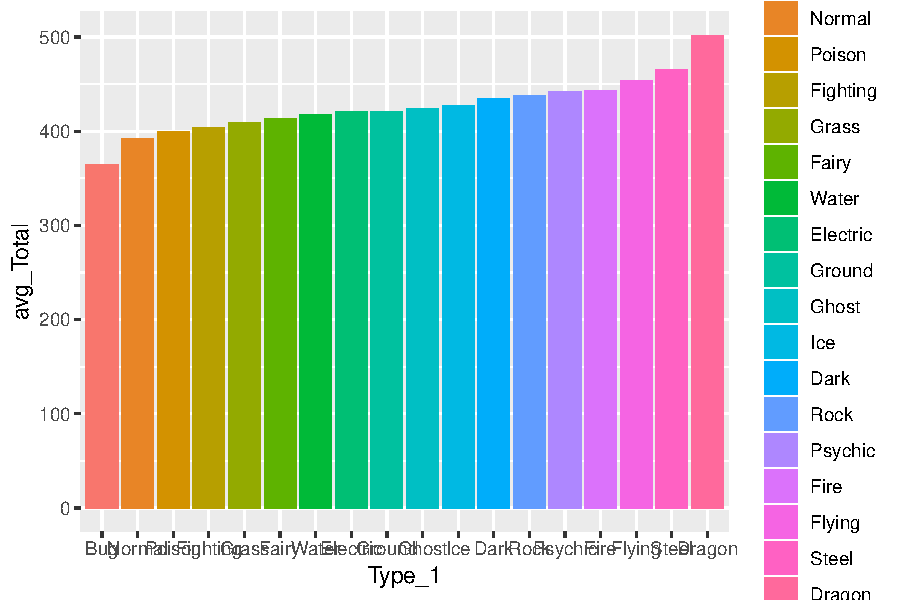
\includegraphics{Figs/unnamed-chunk-2-1.pdf}

\begin{Shaded}
\begin{Highlighting}[]
\NormalTok{pokes }\OperatorTok\StringTok{ }
\StringTok{  }\KeywordTok{group_by}\NormalTok{(Catch_Difficulty, Type_}\DecValTok{1}\NormalTok{) }\OperatorTok\StringTok{ }
\StringTok{  }\KeywordTok{summarize}\NormalTok{(}\DataTypeTok{avg_Total =} \KeywordTok{mean}\NormalTok{(Total)) }\OperatorTok\StringTok{ }
\StringTok{  }\KeywordTok{mutate}\NormalTok{(}
    \DataTypeTok{Type_1 =} \KeywordTok{fct_reorder}\NormalTok{(Type_}\DecValTok{1}\NormalTok{, avg_Total)}
\NormalTok{  ) }\OperatorTok
\StringTok{  }\KeywordTok{ggplot}\NormalTok{(}\KeywordTok{aes}\NormalTok{(}\DataTypeTok{x =}\NormalTok{ Type_}\DecValTok{1}\NormalTok{, }\DataTypeTok{y =}\NormalTok{ avg_Total, }\DataTypeTok{fill =}\NormalTok{ Type_}\DecValTok{1}\NormalTok{)) }\OperatorTok{+}
\StringTok{  }\KeywordTok{geom_col}\NormalTok{() }\OperatorTok{+}
\StringTok{  }\KeywordTok{facet_wrap}\NormalTok{(}\OperatorTok{~}\NormalTok{Catch_Difficulty)}
\end{Highlighting}
\end{Shaded}

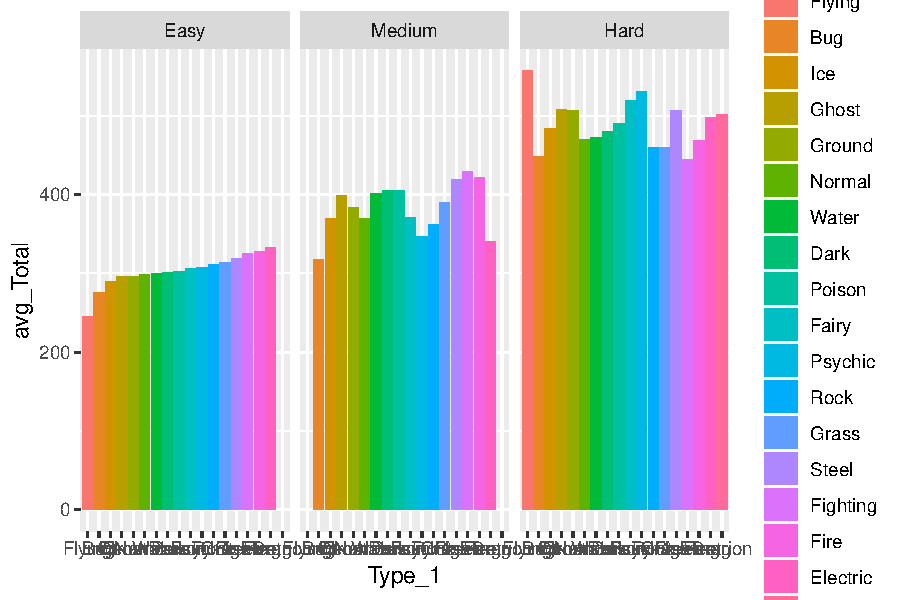
\includegraphics{Figs/unnamed-chunk-2-2.pdf}

\begin{Shaded}
\begin{Highlighting}[]
\NormalTok{pokes }\OperatorTok\StringTok{ }
\StringTok{  }\KeywordTok{ggplot}\NormalTok{(}\KeywordTok{aes}\NormalTok{(}\DataTypeTok{x =}\NormalTok{ Catch_Rate, }\DataTypeTok{y =}\NormalTok{ Total, }\DataTypeTok{color =}\NormalTok{ Catch_Difficulty)) }\OperatorTok{+}\StringTok{ }
\StringTok{  }\KeywordTok{geom_point}\NormalTok{()}
\end{Highlighting}
\end{Shaded}

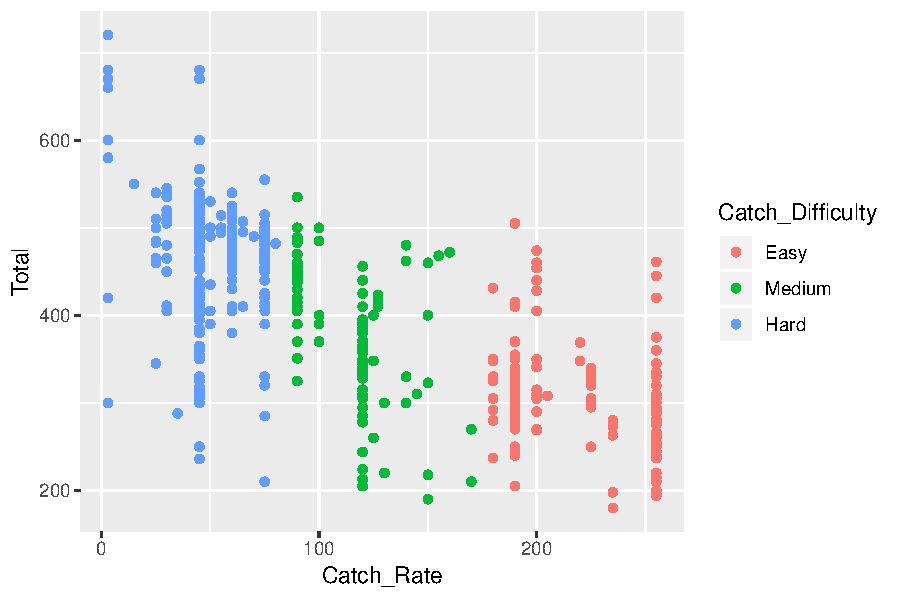
\includegraphics{Figs/unnamed-chunk-2-3.pdf}

\section{2. At least one statistical analysis or
model.}\label{at-least-one-statistical-analysis-or-model.}

\begin{Shaded}
\begin{Highlighting}[]
\CommentTok{# chi-square test}
\NormalTok{pk_type <-}\StringTok{ }\NormalTok{pokes }\OperatorTok
\StringTok{  }\KeywordTok{count}\NormalTok{(Type_}\DecValTok{1}\NormalTok{, Catch_Difficulty) }\OperatorTok
\StringTok{  }\KeywordTok{spread}\NormalTok{(}\DataTypeTok{key =}\NormalTok{ Catch_Difficulty, }\DataTypeTok{value =}\NormalTok{ n) }\OperatorTok
\StringTok{  }\KeywordTok{filter}\NormalTok{(Easy }\OperatorTok{>=}\StringTok{ }\DecValTok{3}\NormalTok{, Medium }\OperatorTok{>=}\DecValTok{3}\NormalTok{, Hard }\OperatorTok{>=}\StringTok{ }\DecValTok{3}\NormalTok{)}
\NormalTok{pk_type }\OperatorTok\StringTok{ }
\StringTok{  }\KeywordTok{select}\NormalTok{(}\OperatorTok{-}\NormalTok{Type_}\DecValTok{1}\NormalTok{) }\OperatorTok\StringTok{ }
\StringTok{  }\KeywordTok{chisq.test}\NormalTok{()}
\end{Highlighting}
\end{Shaded}

\begin{verbatim}
## 
##  Pearson's Chi-squared test
## 
## data:  .
## X-squared = 60.199, df = 30, p-value = 0.000871
\end{verbatim}

\begin{Shaded}
\begin{Highlighting}[]
\CommentTok{# t-tests}
\NormalTok{em <-}\StringTok{ }\NormalTok{pokes }\OperatorTok
\StringTok{  }\KeywordTok{count}\NormalTok{(Type_}\DecValTok{1}\NormalTok{, Catch_Difficulty) }\OperatorTok\StringTok{ }
\StringTok{  }\KeywordTok{filter}\NormalTok{(Catch_Difficulty }\OperatorTok{==}\StringTok{ "Easy"} \OperatorTok{|}\StringTok{ }\NormalTok{Catch_Difficulty }\OperatorTok{==}\StringTok{ "Medium"}\NormalTok{)}
\KeywordTok{t.test}\NormalTok{(n }\OperatorTok{~}\StringTok{ }\NormalTok{Catch_Difficulty, }\DataTypeTok{data =}\NormalTok{ em)}
\end{Highlighting}
\end{Shaded}

\begin{verbatim}
## 
##  Welch Two Sample t-test
## 
## data:  n by Catch_Difficulty
## t = 1.4115, df = 24.959, p-value = 0.1705
## alternative hypothesis: true difference in means is not equal to 0
## 95 percent confidence interval:
##  -1.612490  8.634549
## sample estimates:
##   mean in group Easy mean in group Medium 
##             10.82353              7.31250
\end{verbatim}

\begin{Shaded}
\begin{Highlighting}[]
\NormalTok{eh <-}\StringTok{ }\NormalTok{pokes }\OperatorTok
\StringTok{  }\KeywordTok{count}\NormalTok{(Type_}\DecValTok{1}\NormalTok{, Catch_Difficulty) }\OperatorTok\StringTok{ }
\StringTok{  }\KeywordTok{filter}\NormalTok{(Catch_Difficulty }\OperatorTok{==}\StringTok{ "Easy"} \OperatorTok{|}\StringTok{ }\NormalTok{Catch_Difficulty }\OperatorTok{==}\StringTok{ "Hard"}\NormalTok{)}
\KeywordTok{t.test}\NormalTok{(n }\OperatorTok{~}\StringTok{ }\NormalTok{Catch_Difficulty, }\DataTypeTok{data =}\NormalTok{ eh)}
\end{Highlighting}
\end{Shaded}

\begin{verbatim}
## 
##  Welch Two Sample t-test
## 
## data:  n by Catch_Difficulty
## t = -2.8847, df = 27.061, p-value = 0.007598
## alternative hypothesis: true difference in means is not equal to 0
## 95 percent confidence interval:
##  -21.406927  -3.612681
## sample estimates:
## mean in group Easy mean in group Hard 
##           10.82353           23.33333
\end{verbatim}

\begin{Shaded}
\begin{Highlighting}[]
\NormalTok{mh <-}\StringTok{ }\NormalTok{pokes }\OperatorTok
\StringTok{  }\KeywordTok{count}\NormalTok{(Type_}\DecValTok{1}\NormalTok{, Catch_Difficulty) }\OperatorTok\StringTok{ }
\StringTok{  }\KeywordTok{filter}\NormalTok{(Catch_Difficulty }\OperatorTok{==}\StringTok{ "Medium"} \OperatorTok{|}\StringTok{ }\NormalTok{Catch_Difficulty }\OperatorTok{==}\StringTok{ "Hard"}\NormalTok{)}
\KeywordTok{t.test}\NormalTok{(n }\OperatorTok{~}\StringTok{ }\NormalTok{Catch_Difficulty, }\DataTypeTok{data =}\NormalTok{ mh)}
\end{Highlighting}
\end{Shaded}

\begin{verbatim}
## 
##  Welch Two Sample t-test
## 
## data:  n by Catch_Difficulty
## t = -4.0609, df = 20.485, p-value = 0.0005857
## alternative hypothesis: true difference in means is not equal to 0
## 95 percent confidence interval:
##  -24.237778  -7.803889
## sample estimates:
## mean in group Medium   mean in group Hard 
##              7.31250             23.33333
\end{verbatim}

\section{3. Proper discussion and interpretation of all
work.}\label{proper-discussion-and-interpretation-of-all-work.}

Conclusion:


\end{document}
